%/*% pdflatex -file-line-error -interaction nonstopmode %

\documentclass{article}
\usepackage{graphicx}
\graphicspath{ {./images/} }
\usepackage{amsmath}
\usepackage{amsfonts}
\usepackage{hyperref}
\usepackage{exercises}
\usepackage{amsthm}
\usepackage{yhmath}
\newcommand*{\oldneg}{\mathord{\sim}}

\theoremstyle{definition}
\newtheorem{definition}{Definition}

\setlength{\parindent}{.5in}
\setlength{\parskip}{12pt}

\title{Quiz 3 (pg. 73)}
\begin{document}
\maketitle

\section*{1}
$x^2-4x+5=0\newline\rightarrow 
x=\frac{4\pm\sqrt{(-4)^2-4(1)(5)}}{2(1)}\newline\rightarrow 
x=\frac{4\pm\sqrt{-4}}{2}\newline\rightarrow 
x=\frac{4\pm 2i}{2}\newline\rightarrow 
x=2\pm i\newline\rightarrow 
x=2+i\vee x=2-i$

\section*{2}
$2x^2-8x+1=0\newline\rightarrow 
x=\frac{8\pm\sqrt{(-8)^2-4(2)(1)}}{2(2)}\newline\rightarrow 
x=\frac{8\pm\sqrt{56}}{4}\newline\rightarrow 
x=\frac{8\pm 2\sqrt{14}}{4}\newline\rightarrow 
x=\frac{4\pm\sqrt{14}}{2}\newline\rightarrow 
x=2+\frac{\sqrt{14}}{2}\vee x=2-\frac{\sqrt{14}}{2}$

\section*{3}
$3x^2+5x+4=0\newline\rightarrow 
x=\frac{-5\pm\sqrt{5^2-4(3)(4)}}{2(3)}\newline\rightarrow 
x=\frac{-5\pm\sqrt{-23}}{6}\newline\rightarrow 
x=\frac{-5\pm\sqrt{23}i}{6}\newline\rightarrow 
x=-\frac{5}{6}+\frac{\sqrt{23}}{6}i\vee x=-\frac{5}{6}-\frac{\sqrt{23}}{6}i$

\section*{4}
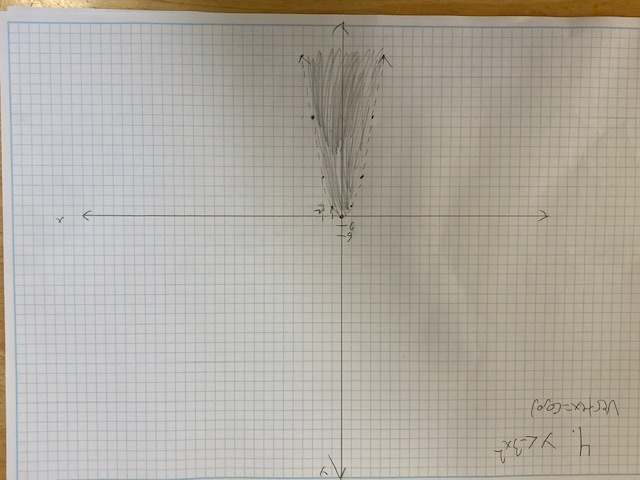
\includegraphics[width = 4in, height = 4in, angle = 180]{quiz3picture1.png}

\section*{5}
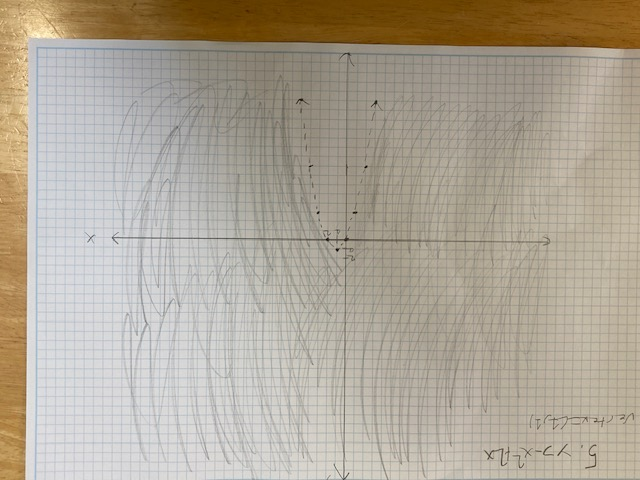
\includegraphics[width = 4in, height = 4in, angle = 180]{quiz3picture3.png}

\section*{6}
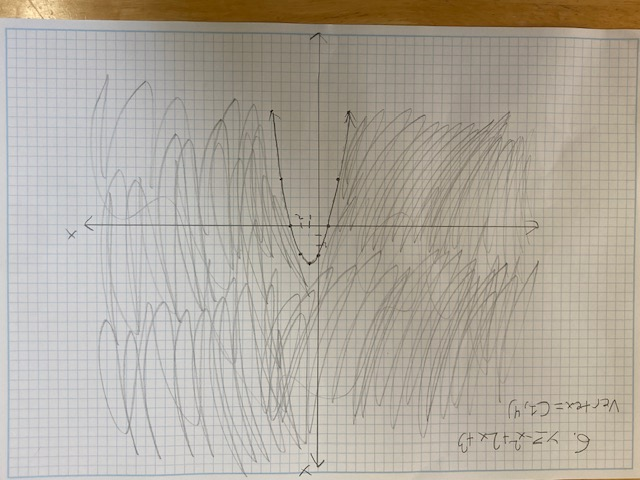
\includegraphics[width = 4in, height = 4in, angle = 180]{quiz3picture2.png}

\section*{7}
$0\ge x^2+5\newline\rightarrow 
x^2+5=0$ (Rewrite in standard form in order to find the intercepts)
$\newline\rightarrow x=\frac{0\pm\sqrt{0^2-4(1)(5)}}{2(1)}\newline\rightarrow 
x=\frac{0\pm\sqrt{-20}}{2}\newline\rightarrow 
x=\frac{0\pm\sqrt{20}i}{2}\newline\rightarrow 
x=0+\frac{\sqrt{20}}{2}i\vee x=0-\frac{\sqrt{20}}{2}i\newline$ Because the graph opens upwards, and we are finding those values such that 
$x^2+5\le 0$, with the given solutions above, we can conlude that the solutions to the inequality are $0-\frac{\sqrt{20}}{2}i\le x\le 0+\frac{\sqrt{20}}{2}i$

\section*{8}
$12\le x^2-7x\newline\rightarrow 
x^2-7x-12\ge 0\newline\rightarrow 
x^2-7x-12=0$ (Rewrite in standard form in order to find the intercepts)
$\newline\rightarrow x=\frac{7\pm\sqrt{(-7)^2-4(1)(-12)}}{2(1)}\newline\rightarrow 
x=\frac{7\pm\sqrt{97}}{2}\newline\rightarrow 
x=\frac{7}{2}+\frac{\sqrt{97}}{2}\vee x=\frac{7}{2}-\frac{\sqrt{97}}{2}\newline$ Because the graph opens upwards, and we are finding those values of $x$ 
such that the $x^2-7x-12\ge 0$, with the above information about the intercepts, we can conlude that the solutions to this inequality are 
$x\le \frac{7}{2}-\frac{\sqrt{97}}{2}\vee x\ge \frac{7}{2}+\frac{\sqrt{97}}{2}$

\section*{9}
$2x^2+2>-5x\newline\rightarrow 
2x^2+5x+2>0\newline\rightarrow 
2x^2+5x+2=0$ (Rewrite in standard form in order to find the intercepts)
$\newline\rightarrow (2x+1)(x+2)=0$ (Factor)
$\newline\rightarrow x=-\frac{1}{2}\vee x=-2\newline$ Because the graph opens upwards, and we are finding those values of $x$ such that $2x^2+5x+2>0$, 
with the above information about the intercepts, we can conclude that the solutions to this inequality are $x<-2\vee x>-\frac{1}{2}$

\section*{10}
For questions $10-12$, recall that the discriminant of a quadratic equation is given by $b^2-4ac$, where $a,b,c$ are all defined from standard form. Hence, 
the discriminant of $2x^2-3x+10=0$ is $(-3)^2-4(2)(10)=-71$. Because the discriminant is negative, $2x^2-3x+10=0$ has two imaginary solutions.

\section*{11}
The discriminant of $-x^2-4x-4=0$ is $(-4)^2-4(-1)(-4)=0$. Because the discriminant is zero, $-x^2-4x-4=0$ has one real solution.

\section*{12}
The discriminant of $x^2-6=0$ is $0^2-4(1)(-6)=24$. Because the discriminant is positive, $x^2-6=0$ has two real solutions.

\section*{13}
Let us recall that the equation:\newline $-16t^2+v_0t+h_0=h$\newline represents the height $h$ of an object dropped from an initial height of $h_0$ at a 
velocity of $v_0$ after $t$ seconds. So, knowing that this problem includes values such that $v_0=30$ and $h_0=5$, an equation representing the path of 
the ball in this problem is $-16t^2+30t+5=0$. To find how long the ball is in the air for, we need to find the positive intercept, as this tells us 
when the ball will hit the ground. We can do this by using the quadratic formula:\newline
$t=\frac{-30\pm\sqrt{30^2-4(-16)(5)}}{2(-16)}\newline\rightarrow 
t=\frac{-30\pm\sqrt{1220}}{-32}\newline\rightarrow 
t=\frac{-30\pm 2\sqrt{305}}{-32}\newline\rightarrow 
t=\frac{15}{16}-\frac{1}{16}\sqrt{305}\vee t=\frac{15}{16}+\frac{1}{16}\sqrt{305}\newline$ Taking the positive intercept, we can conlude that 
the ball is in the air for $\frac{15}{16}+\frac{1}{16}\sqrt{305}$, or about $2.03$ seconds. 
\end{document}
